\chapter[Proposta de Solução]{Proposta de Solução}\label{cap2}

A proposta de solução deste trabalho é um produto interdisciplinar na união dos cinco cursos de engenharia presentes no campus UnB - Gama, com o intuido de resolver os problemas apresentados no capítulo anterior. A proposta inicial de solução é desenvolvimento de um alimentador automático, com capacidade de regarga de bateria via energia solar e de armazenamento de ração para um período rasoável de autonomia. A implementação desta proposta envolve diversas áreas de conhecimento e estará melhor detalhada nas seções seguintes.
A organização da apresentação da solução está baseada em sub-sistemas que integrados resultarão na solução como um todo.

\section{Requisistos do Sistema}
\textbf{FALTA FAZER}
Lista de requisitos de projeto: tanto do cliente quanto dos projetistas
\subsection{Requisitos Eletrônicos}
\textbf{FALTA FAZER}
\subsection{Requisitos Estruturais}
\textbf{FALTA FAZER}
\subsection{Requisitos Energéticos}
\textbf{FALTA FAZER}
\subsection{Requisitos de Locomoção}
\textbf{FALTA FAZER}
\subsection{Requisitos de Software}
\textbf{FALTA FAZER}

\section{Limitações}
Está sessão aborda as limitações do projeto, isto é, o que o a solução não resolverá ou não poderá desenvolver
devido a escolhas ou limitações.

\subsection{Limitações Eletrônicas}
A escolha de todos os componentes eletrônicos utilizados no alimentador estão, basicamente, condicionados ao consumo energético, uma vez que o sistema depende da alimentação de uma bateria que é recarregada esporadicamente durante a atividade solar.

Um fator que poderia ser limitante é a dimensão física dos componentes, que deverão ser alojados dentro de uma carcaça que não ocupe uma dimensão considerável do alimentador. Como a capacidade do tanque de ração está prevista para 300 kg, o volume do ocupado pela parte eletrônica não deve ser preocupante, em vista da relativa baixa quantidade de componentes e sensores requeridos para a atividade do alimentador.

Devido ao produto ser concebido para estar exposto a um ambiente bastante úmido e suscetível à tempestades e movimentação intensa da água, será utilizada uma carcaça que guarda todos os componentes e que deverá ser mantida totalmente selada. Por conta de alguns componentes que aquecem acima do comum, como os drivers do motor, não havendo disponível a circulação de ar para dissipar o calor gerado e refrigerar o circuito integrado , devendo ser dimensionado para operar frio.

\subsection{Limitações Estrutuais}
Componentes como o transportador de alimentos só terá sua efetividade comprovada a partir de testes exaustivos feitos com diferentes granulometrias de ração.

Na parte de isolamento térmico não foi encontrados dados técnicos sobre o produto, apenas dados comerciais, dificultando assim uma comparação mais precisa de soluções possíveis.

\subsection{Limitações Energéticas}
\subsection{Limitações de Software}

\section{Visão geral da solução}

De acordo com o que foi apresentado no termo de abertura do projeto, a solução proposta envolve diversos módulos funcionais, são eles: o alimentador, a base, e o sistema de controle SCADA. A partir de uma visão de alto nível do projeto, como a apresentada na Figura \ref{diagrama}, é possível observar de maneira clara os módulos que deverão se comunicar para garantir o funcionamento do sistema como um todo.

\begin{figure}[H]
 \centering
   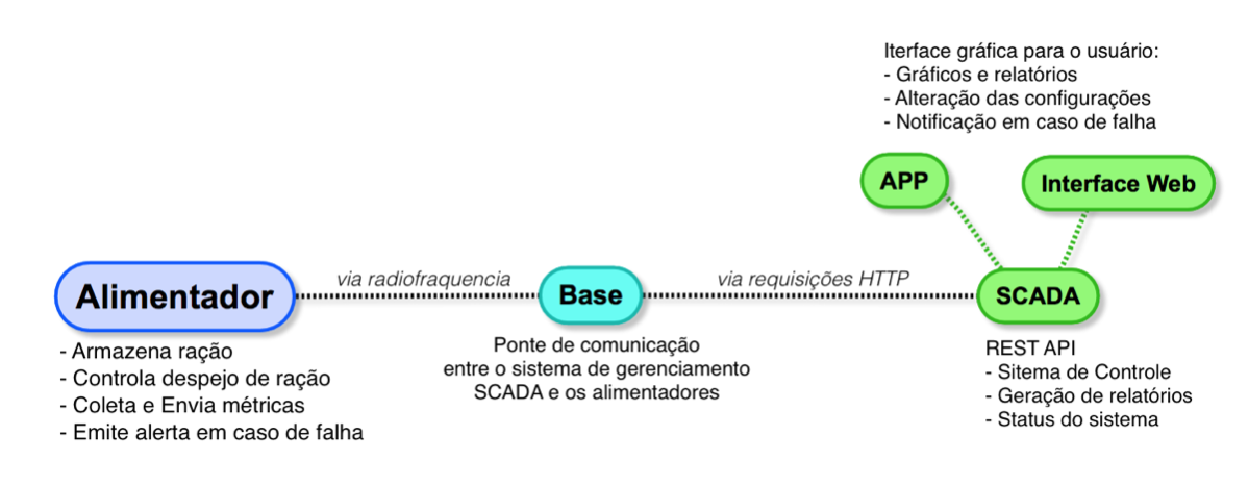
\includegraphics[keepaspectratio=true,scale=0.8]{figuras/digrama_geral.eps}
 \caption{Arquitetura geral da solução}
 \label{diagrama}
\end{figure}

Para garantir que a solução seja responsável, do ponto de vista de situações críticas, como a falha na comunicação entre os alimentadores e base, os alimentadores possuem autonomia de funcionamento, isto é, são capazes de operar independentemente. Tendo por base a configuração presente no equipamento.

Uma vez que o alimentador estará presente no tanque de peixe e este, por sua vez, pode ficar distante da margem, pareceu-se conveniente a utilização de uma via de comunicação de grande alcance(radiofrequência) para se comunicar com um aparelho base responsável por receber informações dos alimentadores e envia-las para o sistema de controle SCADA através de uma rede local.

O sistema SCADA consiste de uma API REST responsável por receber e armazenar os dados dos alimentadores e deve disponibilizar de forma estrutura para os gestores da piscicultura através de uma interface gráfica web e mobile.
